
%\documentclass[journal=no,submission,spthm]{iacrtrans} 
%\documentclass[twoside]{IEEEtran}
\documentclass{llncs}

\usepackage{listings}
\usepackage{color}

\definecolor{dkgreen}{rgb}{0,0.6,0}
\definecolor{gray}{rgb}{0.5,0.5,0.5}
\definecolor{mauve}{rgb}{0.58,0,0.82}

\lstset{frame=tb,
  language=Java,
  aboveskip=3mm,
  belowskip=3mm,
  showstringspaces=false,
  columns=flexible,
  basicstyle={\small\ttfamily},
  numbers=none,
  numberstyle=\tiny\color{gray},
  keywordstyle=\color{blue},
  commentstyle=\color{dkgreen},
  stringstyle=\color{mauve},
  breaklines=true,
  breakatwhitespace=true,
  tabsize=3
}

\usepackage{algorithm}
\usepackage[]{algorithmic}
\usepackage{pgfplots}
\pgfplotsset{compat=1.16}
\usepackage{graphicx}
\usepackage[english]{babel}
\usepackage[utf8x]{inputenc}
\usepackage[T1]{fontenc}
\usepackage{upgreek}
\makeatletter
\newcommand{\ssymbol}[1]{^{\@fnsymbol{#1}}}
\makeatother
\newcommand{\todo}[0]{\textcolor{yellow}{TODO}}
\usepackage[weather]{ifsym}
\usepackage{xcolor,colortbl}
\usepackage{url}
\usepackage{array}
\usepackage{amsfonts}
\usepackage{amssymb}
\usepackage{amsmath}
\usepackage{graphicx}
\usepackage{mdframed}
\usepackage[colorlinks=false, allcolors=blue]{hyperref}
\usepackage[pdf]{graphviz}
\usepackage{subcaption}
\usepackage{cleveref}

\DeclareMathOperator{\numUses}{numUses}
\DeclareMathOperator{\Tab}{Tab}
\DeclareMathOperator{\CB}{CB}
\DeclareMathOperator{\expiry}{expiry}
\DeclareMathOperator{\Encrypt}{Encrypt}
\DeclareMathOperator{\extra}{extra}
\DeclareMathOperator{\rand}{rand}
\DeclareMathOperator{\oldkey}{old\_key}
\DeclareMathOperator{\newkey}{new\_key}
\DeclareMathOperator{\sk}{sk}
\DeclareMathOperator{\SHA}{SHA}
\DeclareMathOperator{\tok}{tok}

\pgfplotsset{select coords between index/.style 2 args={
    x filter/.code={
        \ifnum\coordindex<#1\def\pgfmathresult{}\fi
        \ifnum\coordindex>#2\def\pgfmathresult{}\fi
    }
}}

\newcounter{algoc}
\setcounter{algoc}{0}
\newtheorem{algo}[algoc]{Algorithm}

\newcounter{prob}
\setcounter{prob}{0}
\newtheorem{Problem}[prob]{Problem}

\newcommand{\ph}[1]{\emph{\bf \color{red}~[Paul: #1]}}
\newcommand{\ab}[1]{\emph{\bf \color{blue}~[Agathe: #1]}}
\newcommand{\cn}[1]{\emph{\bf \color{purple}~[Cyrius: #1]}}
%\usepackage{syntonly}
%\syntaxonly

\begin{document}
\pagestyle{plain}
% \title{Generation and security of tokens}
\title{A free-spot tokenization approach for credit card numbers}
\author{The dream team}
\institute{REDOCS 2020}
\maketitle


\begin{abstract}
Internet users are increasingly concerned about their privacy and are looking for ways to protect their data. On top of that, they may rightly fear that companies learn information about them from their online behavior. The so-called tokenization process allows the use of temporary identities managed by a trusted third party from which no personal data about the user can be inferred.
We study in this paper tokenization systems allowing one to hide the banker identity of a customer. We present here a method for generating and managing tokens using a database. We refer to our approach as \lq\textit{free-spot}\rq as it keeps generating new tokens until it finds a free spot to insert it in the table, thus avoiding collisions.
We analyze the security of our tokenization system and prove that it satisfies the specifications of the domain. Finally, we provide measurements from an implementation, that confirms the validity of our approach.
\end{abstract}


\section{Introduction}
% gérer un grand nombre de tokens en un minimum de place
% ajouter dans schéma: signature client + double authentif.
Even under a pseudonym, Internet users leave digital 
8
 fingerprint behind them. All this data can be studied in order to infer information about the user and his behavior. This is notably done on the largest e-commerce platforms and social networks.

In order to reduce this traceability and limit the possible inferences of the data, a proposed approach is to give a temporary identity to the user. This temporary identity, called a token, is delivered by a trusted third-party, the Token Service Provider (TSP), that serves as a proxy masking the user's real identity.

To increase the security of mobile payments, many payment systems today use a technology called \lq tokenization\rq. Tokenization is the process of replacing an existing payment card number with a substitute value (token). This token is used during a payment transaction, allowing the original card number to be kept securely. A Token Service Provider (TSP) is an entity within the payment ecosystem that generates and manages tokens. So it is an entity within the payments ecosystem that generates and manages tokens. For example, TSP associates the original card number with the payment tokens and stores them securely in a token vault. These tokens can only be used in a specific area such as a merchant's website or online channel, which further limits the risk. 

A TSP manages the entire lifecycle of payment vouchers, including the Authorization Host Token Applicant. It does this as follows:
\begin{enumerate}
    \item \textit{Tokenization}: Replaces the \textsc{pan} with a payment token.
    \item \textit{Detokenization}: Converts the token back to a \textsc{pan} using the token vault.
    \item \textit{Token vault}: Establishes and maintains the correspondence between the payment token and the \textsc{pan}.
    \item \textit{Domain management}: Adds additional security by limiting the tokens to be used in specific channels or (retail) domains.
    \item \textit{Identification and verification}: Ensures that the payment token replaces a \textsc{pan} that has been legitimately used by the token requestor.
\end{enumerate}

Issuers, acquirers, and merchants who wish to offer mobile and/or digital payments to their customers can become a TSP. Becoming its own TSP allows full control of the tokenization process: creation, storage, issuance, and management. By having his own TSP, one has full control over digital payments by issuing tokens directly without the intervention of a third party. Therefore, costs are reduced in the long run, as there are no additional fees for payment systems. In addition, the transaction is done on the spot, saving on transaction fees when one is the issuing and acquiring bank. Otherwise, the issuers may use a third-party TSP from payment systems and integrate it with their payment systems.

A concrete use of such Tokenization Systems is found for example in the domain of hiding bank account information. The typical scenario in this context is depicted in Figure~\ref{fig:tokenization-system}. First, the customer requests a token from the Token Service Provider (1), which needs information to identify the user, e.g., its bank data, which is transmitted securely (2). The Token Service Provider generates a token from this data and returns it to the user in a secure manner (3). Then, the user making purchases transmits his token to a merchant site (4). To request the payment, the user contacts the Token Service Provider (5), which confirms the validity of the token and requests payment (6) from the bank to the merchant site (7).

\begin{figure}
    \centering
    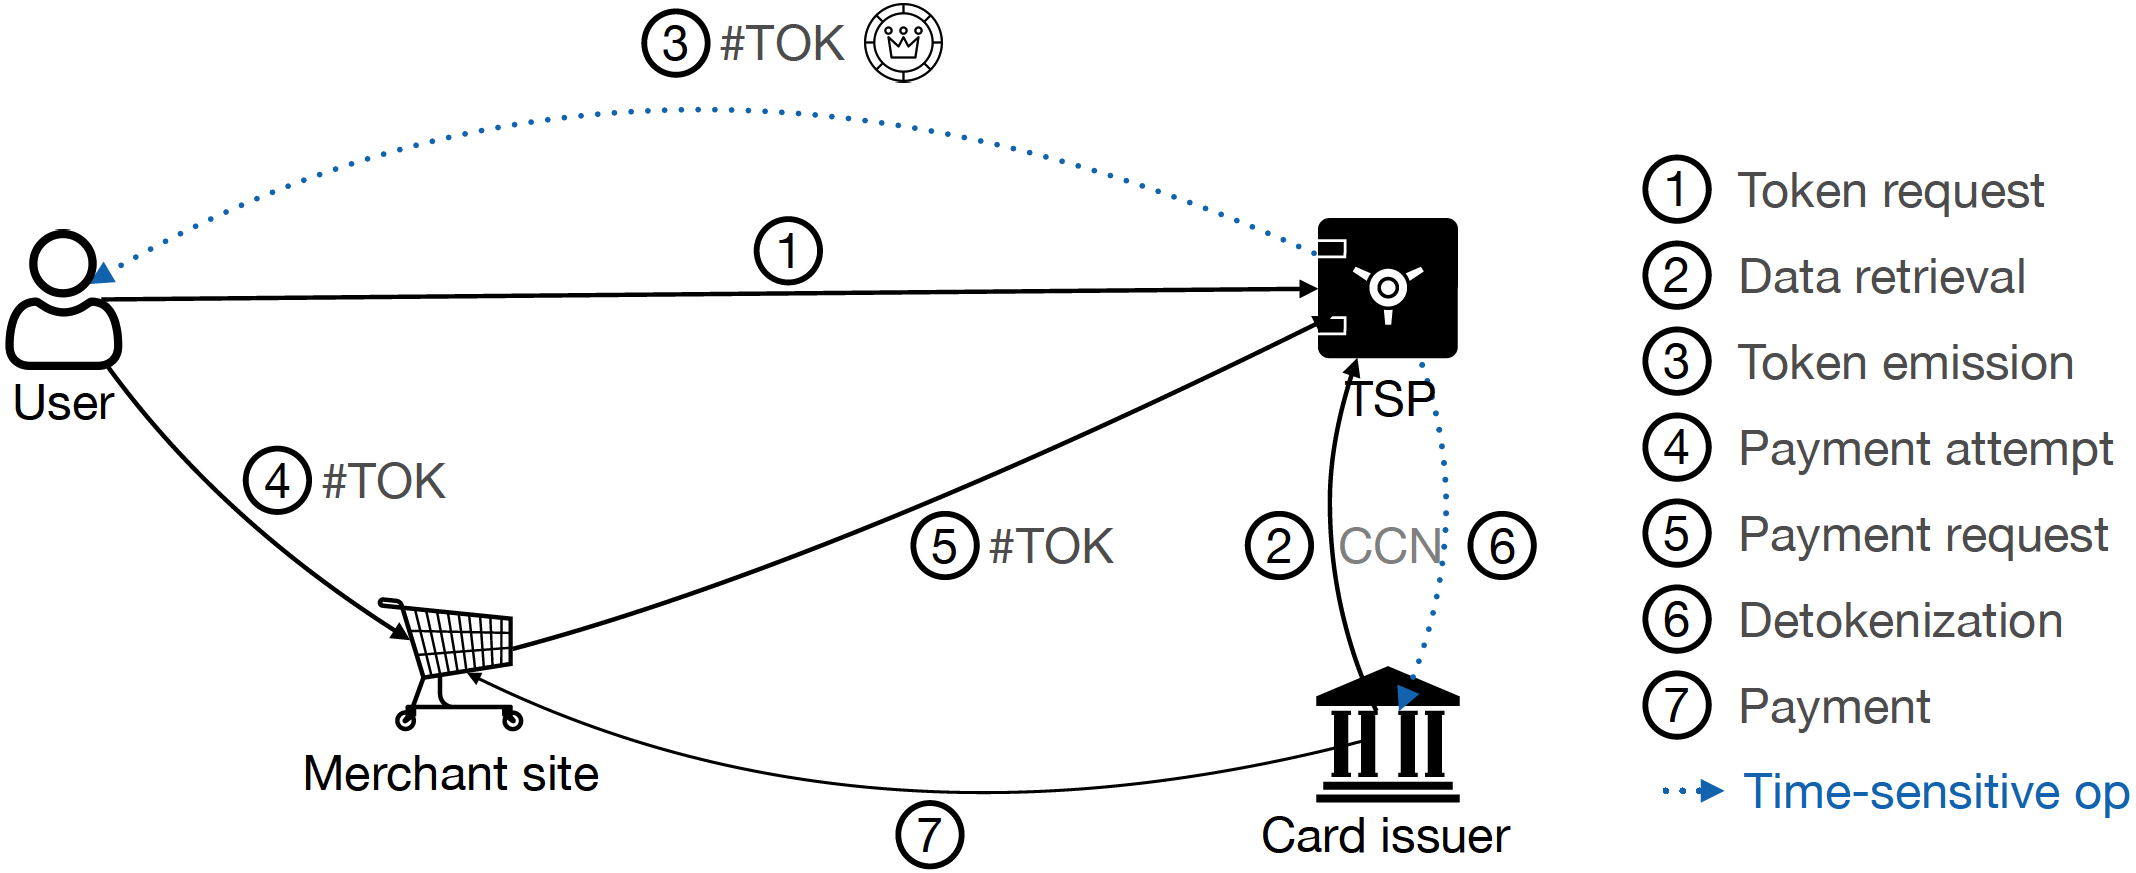
\includegraphics[width=\textwidth]{Tex/Figures/use_case.png}
    \caption{Tokenization system in our use case}
    \label{fig:tokenization-system}
\end{figure}

Credit card numbers (\textsc{ccn}s) are the identifiers that can be found on any payment cards.  These so-called primary account numbers (or \textsc{pan}s) consist of a maximum of 19 digits that identify the card issuer and the cardholder. (\textsc{ccn}s) are usually stored on 64 bits to include the 16 \textsc{ccn}s digits plus the three \textsc{CVC} digits.
They are made up of three main components, in accordance with ISO/IEC 7812-1~\cite{ISO78121}:
\begin{enumerate}
    \item The issuer identification number (\textsc{inn}), which corresponds to the leading 8 numerical digits. %It starts with the Major Industry Identifier (\textsc{mii}).
    \item The individual account number, which can be of variable length -- between 1 and 10 digits.
    \item A check digit computed from all the preceding digits of the \textsc{pan} using the Luhn algorithm, also known as the \lq\textit{modulus 10}\rq algorithm \cite{Luhn1960}.
\end{enumerate}

The individual account number is usually 4-digit long, which amounts to a total of 16 digits in for the \textsc{pan}. In the considered instance, the structure of the tokens slightly deviates from the conventional format: the first four digits identify the card issuer and the last four digits are fixed, leaving 8 digits open to identify a token. \ph{demander a marius une vraie justification?}

The specifications for the tokenization systems are listed hereafter.
\begin{enumerate}
    \item \label{item-spec-disting} \textit{Unicity}: Each token should be attributed to at most one user at any given time.
    \item \textit{Expiry time}: A token has a maximal number of uses and an expiry date.
    \item \label{item-spec-format-ccn} \textit{Formatting}: The format of the token should be identical to \textsc{ccn}s 
    \item \textit{Identical distribution}: The distribution of the tokens should match the one of \textsc{ccn}s. \textcolor{blue}{verifier que les INN sont uniformes @marius}
    \item \label{item-spec-linkable} \textit{Unlinkability}: Tokens should not be linkable to one another, or to a user.
    \item \label{item-spec-time} \textit{Timeframe}: Tokenization and Detokenization computation times should not exceed a given timeframe value denoted $Tf$. In this paper, we consider $Tf$ to be 100 ms.
    \item \textit{Unforgeability}: An adversary should be unable to forge an invalid token.
\end{enumerate}

\noindent\textbf{Our contributions.}
In this paper, we focus on \textsc{ccn}s tokenization systems. We take a look at different possible solutions to create a tokenization system complying with the specifications. We propose a statistical approach that guarantees the Tokenization to succeed in the given timeframe with overwhelming probability. We propose a proof of concept implementation and study its memory and time performances.
Additionally, we study the possibility to add a database for compliance with extra audit requirements. We look at the compromise between the token unforgeability and the maximal number of valid tokens at any given time.

\smallskip

\noindent\textbf{Organization of the paper. }
Section~\ref{sect:background} contains the study of possible solutions for tokenization systems, knowingly the use of Format Preserving Encryption and the use of a blockchain.
Section~\ref{sect:method} presents our approach to the problem. We study the impact of different parameters on our system and give a proof-of-concept implementation and benchmark results.
Section~\ref{sect:conclu} draws conclusions from our work.


\section{Background and related work}\label{sect:background}

In this section, we present the related work on static pre-compute tables, format-preserving encryption (FPE), and space-efficient data structures. We then position our contribution with respect to the described related work. Note that we also considered of a blockchain to proceed to tokenization and detokenization in a secure way with no central authority, and present it in the appendix.

\subsection{Static pre-compute tables}

In 2012, Voltage Secure proposed a way of generate and use token \cite{Voltage}, according to the Payment Card Industry Data Security Standard (PCI DSS) requirements. Voltage proposed to compute a static table with all possible tokens. When a tokenization is needed then a token is randomly associated to the card number. With a good random generator and a good management of the table where the tokens are stored this solution is completely in accordance with the PCI DSS and allows a quick tokenization. 
\par However, Voltage does not evoke the encryption of the static table and the cleaning of the table is not mentioned. This could be a problem if the number of $10^8$ tokens used is reached. Moreover this technique allow a quick tokenization but could be a problem if the size of the token increases. In that case the table that have to be stored would be bigger and bigger.
\par Our proposition allows to have a dynamic table which is more portable. Moreover we proposed a way of cleaning the table by given a expiration date and a maximum number of uses for each token. Hence, our system allow to deal with the limited number of tokens available in the same time a assure the security of the data gave by the client.
% In \cite{Voltage}, if the a table is fool then an another is generated. This technique allow to use same token in the same time for different credit card but it increase the time of detokenization because more verification are needed to found the goo card numbers. Moreover this implies that there will be more and more table in time if they are not cleaned.

\subsection{Format Preserving Encryption}

Another possibility for the generation of tokens is the use of Format-preserving Encryption (FPE) \cite{Bellare2009}. For simple formats such as the 8 open digits in \textsc{ccn}s, it can be seen as a Pseudorandom Permutation of the set of values of correct format indexed by a key. The key space can be much greater than the space of correct values. The goal of FPE is to avoid the need for a database. The natural use of FPE is to encrypt the 8 open digits of the bank card as the 8 open digits of the token. The validation of the token is then done by decrypting the 8 open digits of the token to retrieve a card number to transmit to the bank for payment. If the token given by the merchant to the TSP is not correct, the corresponding bank account should be invalid.

For now, the domain size is still big enough to not be in reach of some attacks on \textit{small domains}. For example, in \cite{attacksFPEsmallDomains}, attacks are provided on domains up to 8 bits. Following the attacks discovered in \cite{FPEattacks}, the National Institute of Standards and Technology (NIST) recommends using domains of at least one million elements \cite{NistFPErecommandations}. With a one hundred million domain, the \textsc{ccn}s  are still out of reach for now, but this should be a concern for a long-lasting system.

The first limitation found in the use of FPE is that the map from users to the 8 open digits is not bijective, since two banks with different fixed digits can issue the same open digits to two different users, e.g., John Doe 5555 1234 5678 5555 and Michel Dupont 8888 1234 5678 8888. Such a scenario would imply that the tokens generated by these users would always be the same, so that these two users cannot have tokens issued with the same key. Another possibility is to have an injective map from card issuers to Token Service Provider that would avoid this type of conflict.

Supposing that the indexing secret keys are changed regularly, cases would happen where two different card numbers with two different keys yield the same token. In this case, in the verification phase, it would be impossible to differentiate the two tokens (see Specification~\ref{item-spec-disting}). Additionally, the pairs (token, secret key) should be kept in a database in order to know the key that deciphers a given token. This defeats the purpose of using FPE.

On the other hand, if we keep the same secret key across time, it opens the possibility for attackers to trace a token number, since it is permanently linked to the card number. This would not comply with Specification~\ref{item-spec-linkable}.

One could also think of using FPE on a smaller space, i.e., 7 digits, so that some space would be left for differentiating conflicts between two uses of the same token, either if it was issued from two different keys or two different users. The latter case can happen since 7 out of the 8 open digits can be the same for many users. Anyway, the number of collisions that can be differentiated with the extra digit is lesser than the number of possible collisions if the keys change. A good token differentiation would require extra space that cannot be contained in the given format (Specification~\ref{item-spec-format-ccn}). Additionally, the domain becomes closer to the NIST limit of small domains.

To summarize, the use of FPE would either create collisions or require a database. In the latter case, it just creates an overhead that can be avoided with a classical database.

\subsection{Space-efficient data structures}

Different hashing strategies exist to resolve collisions in hash tables:
\begin{itemize}
    \item \textbf{Closed addressing} strategies rely on additional data structures to store all elements with hash collisions, e.g., with linked lists or binary search trees, as separate chaining.
    \item \textbf{Perfect addressing} strategies choose hash functions so that collisions cannot happen, and rehash or move elements when they do. Bloom and Cuckoo filters \cite{Bloom1970} are two space-efficient probabilistic data structures used for approximate set membership. They are designed to check whether an element belongs to a set (here the hash table) or not. They enable one: \textit{1)} to know with certainty that an item does not belong to the table (thus there are no false negative matches); and \textit{2)} to assess the probability that an item belongs to the table (thus false positive matches are possible). Therefore, duplicate values can be avoided as one rehashes elements when there is a collision. However, the number of false positives increases with the size of the table. Unlike Bloom filters, Cuckoo filters propose the advantage to support item deletions.
    \item \textbf{Open addressing} strategies store duplicate values into the same hash table. Such techniques include linear probing, quadratic probing, and double hashing.
\end{itemize}

A major limitation of hashing tables relies on the impact of the load factor on the performances of the system. The load factor is defined as the proportion of slots in the hash table that are used; in other words, the hash table size should be at least $x$ times greater than the number of keys, with $x$ depending on the hashing strategy. When it increases towards 100\%, the number of probes required to find or insert a given key rises dramatically and then requires the expanding of the table. Once the table becomes full, open addressing algorithms may even fail to terminate. The load factor is traditionally capped at 80\% (for which the hash table size would be equal to 1.25 times the number of keys), but often set to 50\% for open addressing strategies, and up to 100\% for separate chaining.
For the cuckoo filter, there is no condition on the table size, but rather on the maximum number of displacements (estimated to 500 operations in \cite{Fan2014}), after which the procedure of recursively finding a vacant bucket becomes unproductive. Several Bloom filter variants exist to address the deletion of items that is not possible by default. However, this incurs a rising in space to retain the same false positive rate as a space-optimized Bloom Filter. Counting Bloom filters \cite{Tarkoma2012} are 3 to 4 times larger, while $d$-left counting Bloom filters \cite{Bonomi2006} use 1.5 times space.

\subsection{Our contribution}

% related to static pre-compute tables
% on clean: réutilisation de tokens, pas de notion de réutilisation
% 13, 14 et 16 du premier papier redocs

% related to FPE

% related to space-efficient data structures
One essential requirement of our algorithm is its scalability, thus we should avoid relying on hash tables whose too high load factor would cause performance degradation. Therefore, we design in our implementation the use of an exact table. The fact we cannot find duplicate values exempts us from the use of a hash table. Unlike using hash tables, the size of our table is strictly equal to the number of keys. In our system, we rely on a function that keeps generating new tokens if one already belongs to the table in order not to handle the storage of duplicate values. Otherwise, we would need to add a parameter to differentiate between two identical token values from two users. For instance, we could use the customer's signature containing its name, identifier, or a personal signature. An alternative version of our algorithm would consist in leveraging hash tables to handle the storage of duplicate values. In addition to hash tables, sketches such as Bloom and Cuckoo filters are both fast and compact space-efficient data structures that produce lower space overhead than hash tables.
Variants of these filters exist to dynamically adapt the size depending on the number of stored elements, so that the size of the table varies with the number of stored elements. In our current implementation, the default size of the table is the maximum number of elements (i.e., set to $10^8$ in our implementation), no matter the number of elements effectively contained. A variant of bloom filters known as scalable Bloom filters \cite{Almeida2007} is designed to adapt dynamically to the number of stored elements while keeping a minimum false positive probability. In the future, one could imagine that card numbers and tokens would cover $m$ digits, with $m$ greater than 8 as in our current implementation. In this case, adapting the size of the table to the number of stored values would save significant place, compared to allocating space for a table containing $n_{\max} = 10^m$ entries by default, no matter the number of elements effectively stored.

\section{Our free-spot tokenization method}\label{sect:method}

\cn{TODO}
In this section, we introduce our collision-resistant tokenization process. In particular, we study the impact of several parameters on our system and give a proof-of-concept implementation as well as benchmark results.

\subsection{System overview}

In this section, we detail the algorithms of the Token Service Provider. The basis of our approach is the creation of a table in RAM indexed on the token numbers, which consists of $n_{\max}$ rows. To retrieve the data from a token, we thus have to consult the correct row from the table corresponding to the id of the token that has to be used. A row is thus composed of:
\begin{itemize}
    \item a card number $\#\CB$, stored on 64 bits to include the 16 \textsc{ccn}s digits plus the three \textsc{CVC} digits.
    % This is necessary for the transaction to proceed, especially during the detokenization step. 
    \item a random number $\rand$ used to generate the token (32 bits). It allows the verification of the row during the \textit{Clean\_table} operation.
    \item a timestamp $\expiry$, which could be expressed in seconds and thus stored over 32 bits, or expressed with a larger range and stored over 64 bits. It indicates the expiry date of the token.
    \item a counter $\numUses$ of the remaining uses of the token. An 8-bit integer is enough for the predicted use of the tokens.
\end{itemize}

The table should be created contiguous in memory so that the access to the $n^\text{th}$ element could be done by calculating the offset from the first element. This way, tokens are basically indexed by their value. This allows keeping a constant access time for lookup while keeping a minimal database space (Specification~\ref{item-spec-time}). For security purposes, it is also recommended that the database should be encrypted via a secret key. We assume all randomness generators to be cryptographically strong.

\subsection{Description of the functions}

The three following functions enable one to complete the whole tokenization and detokenization process, as well as the token storage in a table and its maintenance. The tokenization (\textit{Token\_request}) and detokenization (\textit{Token\_payment\_request}) operations are performed whenever an customer sends a request to get a token from his card number, while the cleaning of the table (\textit{Clean\_table}) is executed to a rate defined by the administrator, e.g., once a week. Hereafter follows a detailed description of each of the processes.

\textbf{Tokenization:} The tokenization process consists in generating a token $\tok$ from a card number $\#\CB$. It also implies to store the data concerning the user in order to proceed to futures payments. The algorithm \textit{Token\_request}$(\Tab, \#\CB , \numUses, \expiry, \extra, \sk)$ takes as input the table $\Tab$, the credit card number of the user $\#\CB$, the maximal number of uses of the token $\numUses$, a timestamp $\expiry$ corresponding to the validity limit of the token, any extra information $\extra$ that it could be useful to retrieve at the time of detokenization, and the system's secret key $\sk$. The algorithm picks uniformly a 32 bit $\rand$ and computes the following, given $n_{\max}$ the number of entries by default in the table: 
$$\tok = \SHA_{224}(\rand) \mod n_{\max} $$

This way, a token is generated by hashing the random number $\rand$ and reducing it to the token space by carrying out a modulo $n_{\max}$ operation on it. Then, it checks whether $\tok$ corresponds to an empty row of the table. If the same token already exists and is valid, then the process restarts with a fresh $\rand$ value until a new token is generated. When the row is empty, it inserts $\textit{Encrypt}_{\sk} (\#\CB | \numUses | \expiry | \rand | \extra)$ in $\Tab$. This $\tok$ is then formatted properly to follow the \textsc{ccn}s format (starting digits and checksums are added). The algorithm outputs the completed token. If no valid token has been found within the given timeframe $Tf$, the process terminates.

%  ajouter dans token\_request signature du client / 
% fonction à part verif_signature, appelée par token\_request, e.g., sur 8 bits --> RSA
Simultaneously, the algorithm \textit{Verify\_signature} is called by \textit{Token\_request} and aims to verify the client's signature stored on 8 bits. The RSA public-key cryptosystem is widely used for secure data transmission. The user must first create and publish a public key based on two large prime numbers, along with an auxiliary value. The prime numbers are kept secret and stored on the client side. When receiving a tokenization request, the bank must first verify the client's authenticity: the client is asked to sign his messages with his prime numbers, then the bank is able to decipher them using the client's public key and check that the signature corresponds to the client. We further detail this method as well as multi-factor authentication in Section \ref{sect:unforgeability}.

\textbf{Detokenization}: The detokenization process consists in retrieving a credit card number $\#\CB$ from a token $\tok$. The algorithm \textit{Token\_payment\_request}$(\Tab, \tok, \sk)$ takes as input the table $\Tab$ and the token $\tok$ to verify. It checks whether the table row indexed by $\tok$ is empty or not. If it is empty, the token is invalid and the algorithm stops, otherwise, the row is deciphered to retrieve $(\#\CB | \numUses | \expiry | \rand | \extra)$. If $\expiry$ is lesser than the time of computation, the row is deleted and the algorithm stops. Else, the \textsc{ccn} is then returned to the bank. Additionally, $\numUses$ is decremented, if it reaches 0, the row is deleted. The row is kept encrypted in the database.

\textbf{Cleaning the table:} The table has to be cleaned regularly in order to allow the reuse of the token. It is important to allow the reuse of tokens because there are only $n\_{max}$ possible valid tokens that can be used at the same time. To perform a cleaning, each row of the table is checked. The algorithm \textit{Clean\_table}$(\Tab,\sk)$ takes as input the table $\Tab$. For all rows, it deciphers the row to retrieve $(\#\CB | \numUses | \expiry | \rand | \extra)$. The number of remaining uses and the expiry date are verified. If the validity date has passed or if the maximum number of times the token has been used is reached, then the row is erased. This operation should be executed periodically according to the expected quantity of decaying tokens. In addition, if the information needs to be retained for possible auditing, then the information is moved to a database specifically designed to keep track of past tokens and transactions. The algorithm \textit{Clean\_table} checks the following:
\begin{itemize}
    \item Whether $\#\CB$ is a valid \textsc{ccn} by verifying the checksum of the \textsc{ccn}.
    \item Whether $\numUses$ is greater than zero.
    \item Whether $\expiry$ is a date in the future
    \item Whether the $\SHA_{224}(\rand)\bmod n_{\max}$ is the index of the row.
\end{itemize}
In any of these cases, the row is invalid and so is deleted.

Note that for additional security, we can detect modifications in the table to all fields except $\numUses$. For this, Token\_request is modified to hash $(\#\CB | \expiry | \rand | \extra)$. The Clean\_table function checks whether this value is the correct index of the row. If this is not the case, that means that a field changed. Since the value of $\numUses$ changes by design, it cannot be included in this verification process.

Also, keeping the same secret key for a long time can be insecure, notably for social engineering attacks. In order to change regularly the secret key, Clean\_table may also be used as a key updater by taking as inputs $\oldkey$, $\newkey$. Each row is deciphered with $\oldkey$, and after normal operations, the row is inserted enciphered with $\newkey$.

\subsection{Proofs of security}\label{sect:proof}

We prove that given a correct set of parameters, each specification is validated by our approach. Note that in our implementation, we choose $n_{\max}$ equal to $10^8$ corresponding to the 8-digit token numbers and and $Tf = 400,00$ based on results from \texttt{openssl} speed tests.
\begin{enumerate}
    \item \textit{Each token should be attributed to at most one user at any given time.} This is validated by the fact that Token\_request only returns a non-existing token.
    \item \textit{A token has a maximal number of uses and an expiry date.} This is guaranteed by the verification process during Token\_payment\_request and the fact that $\numUses$ is decremented after each use.
    \item \textit{The format of the token should be identical to \textsc{ccn}.} This is done by the formatting step at the end of Token\_request.
    \item \textit{The distribution of the tokens should match the one of \textsc{ccn}.} Any newly issued token has a number taken from a distribution indistinguishable from a uniform distribution. Since the remainder of $2^{224}$ modulo $n_{\max} = 10^8$ is $10,249,216 \approx 2^{23.3}$, the chance of picking an element that would cause a difference from the uniform distribution is $\frac{2^{23.3}}{2^{224}} = \frac{1}{2^{200.7}}$, which implies that there is no distinguisher from the uniform distribution up to a security parameter of 200. \ab{On utilise 256 pour lambda par la suite} \cn{bien vu, et il faut que l'implem fasse ça bien aussi, pour le moment on jette des bits à la poubelle mais le desequilibre est donc plus grand... }
    \item \textit{Tokens should not be linkable to one another, or to a user.} Because we added random values into the hash, there is no information deductible from multiple tokens.
    \item \textit{Tokenization and Detokenization computation times should not exceed a given timeframe $Tf$ value.} We can guarantee the probability of failure to deliver a new token up to an arbitrary high-security parameter. However, the implementation and the value of $Tf$ have an impact that we quantified in the upcoming paragraph. 
    
    \item \textit{An adversary should be unable to forge an invalid token. } Without modification of the overall tokenization scheme as presented in \cite{ref}, a merchant site could submit a random illegitimate token and request a payment. By doing this, it would have a probability to "land" on an existing token equal to the number of currently valid tokens divided by the total number of tokens. In a token space of $10^8$, this causes a lot of design constraints. However, we propose a modification of the tokenization scheme presented in \cite{otherref}.
    
\end{enumerate}

\subsubsection{Additional proof on the probability of failing to generate a token}\ph{wip}

Let us consider a token space of size $n_{\max}$, the number of already generated tokens $n$ and the number of tries $T$ to generate a new token that can be done in the given timeframe $Tf$. We study the maximum $n$, such that the probability of a failure to create a new token is smaller than $2^{-\lambda}$, where $\lambda$ is the security parameter. The probability of failure is the probability of obtaining consecutively $T$ already existing tokens, which happens with a probability of $\frac{n}{n_{\max}}$. Thus we obtain the following inequalities:
\begin{align*}
\bigg(\frac{n}{n_{\max}}\bigg)^{T} &<\frac{1}{2^\lambda}\\
n^T &<\frac{n_{\max}^T}{2^\lambda}\\
\log_2(n) &<\frac{\log_2\bigg(\frac{n_{\max}^T}{2^\lambda}\bigg)}{T}\\
\log_2(n) &<\frac{T\times\log_2(n_{\max})-\lambda}{T}\\
n &<2^{\log_2(n_{\max})-\frac{\lambda}{T}.}
\end{align*}

\subsubsection{Unforgeability}\label{sect:unforgeability}

We propose hereafter a mechanism to prevent the risk of an attacker that would forge tokens. When the Token Service Provider receives a token from the merchant site, it must first verify the user's identity. One possibility to do so is to ask the merchant site for a signature containing the user's information to verify the user's identity. If this signature is cryptographically secure there is no way to link signatures to one another or to the user issuing them.

Another possibility to reach this property is to rely on multi-factor authentication. Basically, a randomly generated token has $\frac{n}{n_{\max}}$ chances to effectively belong to the table. A good protection mechanism can require an interaction with the user possessing the legitimate token. The bank can verify the identity of the user through multi-factor authentication. A basic implementation would consist in asking the user to manually validate the operation from his/her own device, in order to claim his/her identity and thus validate the transaction.
With this verification, a legitimate user could validate his spending to his bank without transmitting information to the merchant site, while someone that would like to forge tokens would be easily detected.

\subsubsection{Database audit}

In addition to the storage of token values in the table, we consider the use of an external database for permanent data storage. It would allow the sustainability of our system by storing the history of transactions, through not time-sensitive operations. Two types of operations could be performed, as: \textit{1)} logging every operation into the database, and \textit{2)} data cleaning that would be performed, e.g., once a week, to remove the tokens whose validity time is expired and storing them in the database as well.

\section{Evaluation}

We decided to use the C language to have good memory management. Good memory management allows us not only to reduce the amount of RAM used, but also to reduce the token generation time by decreasing the number of bits to be covered.
% We performed our experiments on a 2017 MacBook Pro with 2.3 GHz Intel Core i5 Processor and 16GB RAM. \ab{Diane: mettre à jour avec les specs du serveur}
For the sake of reproducibility, our source code is publicly available in the appendix.

\subsection{RAM utilization} 

The theoretical amount of RAM usage depends on the encryption design of the table. Depending on the security requirements, one can decide whether to encrypt the table or not. If it is the case, the table would be encrypted with Advanced Encryption Standard (AES) and 128-bit blocks because ... \ab{add justif + ref}. Since the data are stored on 162 bits, the encryption would be done on 2 blocks of 128 bits. In addition, as $n_{\max} = 10^8$ rows have to be stored, $25.6$GB of RAM are necessary for the storage of the encrypted table. If we choose not to encrypt the table, only $16.8$ GB of RAM are used for storage.

Since our implementation uses C structures, our table is a table of structures and is therefore stored on SSD memory and not in RAM. Hence, the total amount of RAM usage is equal to $3.2$GB only. Each structure, i.e., each row, uses only 32 bits of RAM, thus it represents $3.2$GB of RAM usage for the $10^8$ rows. However, if the table is encrypted, the structure can not be used efficiently and the data must be stored in RAM. In that case, the theoretical number of RAM usage, i.e, $25.6$GB, is reached.

\subsection{Filling rate}

Given the formula $n <2^{\log_2(n_{\max})-\frac{\lambda}{T}}$ found in Section \ref{sect:proof}, the theoretical filling rate of the table before a failure occurs with a probability over $2^{-256}$ and 400,000 tries per $Tf$ equals to $99.92\%$. In other words, the probability of failure becomes larger than $2^{-256}$ when the table is more than $99.92\%$ filled. Our experiments show that the average filling rate before a failure occurs is about $99.998\%$. This is due to the fact that even after $99.92\%$ of filling, there is still a high chance that valid tokens are generated.

The timeframe used is $100$ms, that is to say, that a failure occurs when a valid token has not been generated in $100$ms. The number of trials that our implementation gives per timeframe is about $7220$. By using a faster random generator, this number would be higher. The random generator does not have to be a cryptographic generator, but only to guarantee the uniformity of the generated numbers. \textcolor{purple}{contre exemple: un compteur a une distrib uniforme et est attaquable}

As a result, we show that the theoretical filling rate $n$ of the table must be lower than $2^{\log_2(n_{\max})-\frac{\lambda}{T}}$ in order to insert a new token without collision within the given timeframe $Tf$. By using $Tf = 400,000$ and $\lambda=128$, with this formula, one can achieve a theoretical table filling rate equal to 99.92\%, as illustrated in Figure~\ref{fig:3d-plot}. In addition, the Figure shows the table filling rate value obtained through our assessment. For $Tf=7,221$ and $\lambda=256$, the real table filling rate obtained is equal to 97.57\%.
% \ab{Le schéma représente le filling rate théorique ou réel ? Comment sont obtenus/choisis lambda et Tf ?}

\begin{figure}
    \centering
    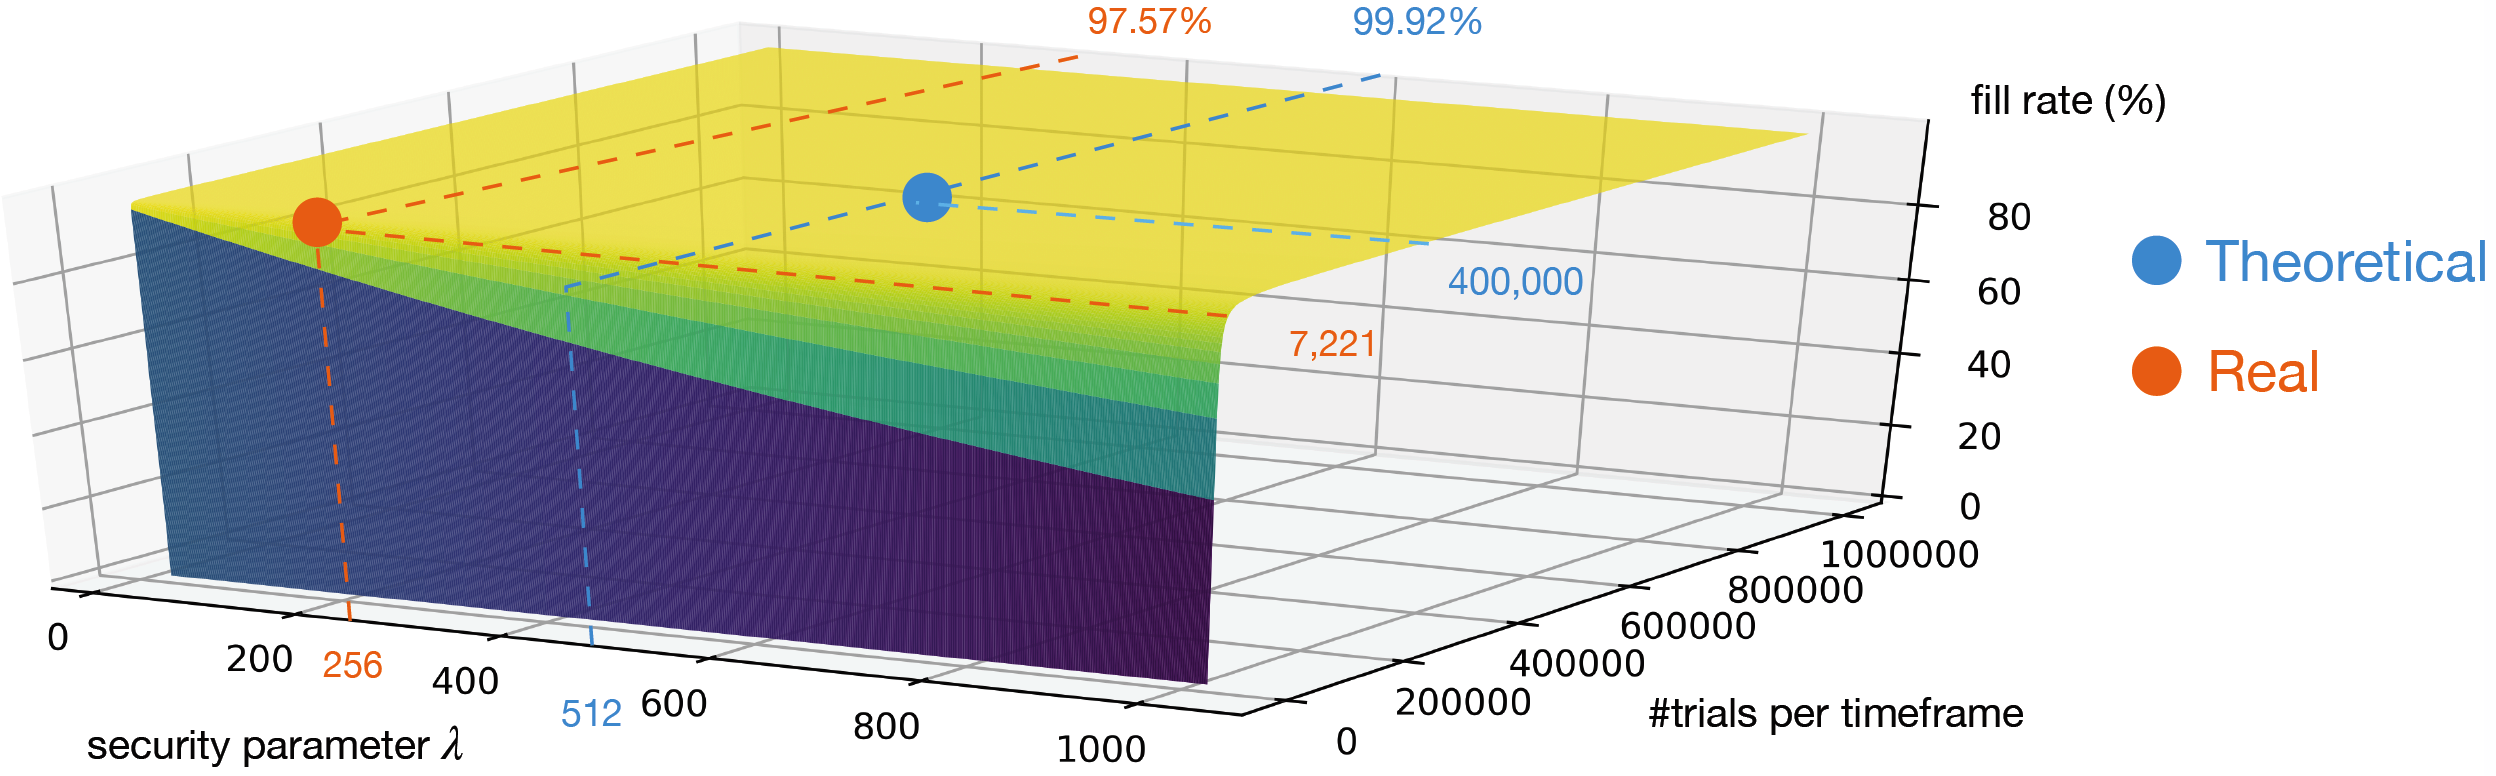
\includegraphics[width=\textwidth]{Tex/Figures/3d_plot}
    \caption{Theoretical and real table filling rates values, achieved for several combinations of $\lambda$ and $Tf$.}
    \label{fig:3d-plot}
\end{figure}

\subsection{Detokenization and cleaning table time}

\section{Conclusion}\label{sect:conclu}
In this paper, we propose a solution for tokenization systems for Credit card numbers. This system is based on the possibility to have the full table of tokens in RAM and so computations are fast enough to guarantee a tokenization without collision. As a result, we found that we can achieve token generation and storage within the given timeframe until the table filling rate reaches to 99.92\% theoretically, and 97.57\% according to our assessment.
We additionally study the inclusion of extra mechanisms to prevent against counterfeited tokens, to allow for a database audit, and to reduce the table size.

% \section*{Acknowledgments}
% This work has been accomplished during the french working session REDOCS’20. REDOCS stands for \textit{Rencontre Entreprises DOCtorants en Sécurité}. It is a one week event, where cybersecurity PhD students are working in groups to solve real life problems proposed by industrial companies. The authors of this work would like to thank the GDR Security for organizing the event. Special thanks go to Pascal Lafourcade and Olivier Blazy who guided them during the whole week. The authors also thank Be-Ys for having proposed this project. They particularly thank Marius Lombard-Platet for having supervised this work.

\section*{Appendix}\label{appendix:code}

We provide hereafter the source code for tokenization, detokenization, and cleaning of the table, that we used for our evaluation. We also insert a study on whether applying a blockchain to our system would be feasible.

\textbf{Source code}

\begin{lstlisting}
#include <string.h>
#include <stdint.h>
#include <time.h>
#include <signal.h>
#include <sys/time.h>
#include <unistd.h>
#include <math.h>
#include <pthread.h>
#include <time.h>
#include <stdio.h>
#include <stdlib.h>
#include <openssl/sha.h>
#include <openssl/rand.h>
#include <openssl/aes.h>
#include <openssl/conf.h>
#include <openssl/evp.h>
#include <openssl/err.h>

#define aesSize 256
#define HASH_LENGTH 2*SHA224_DIGEST_LENGTH+1

#define TIMEFRAME 0.1
#define LIFESPAN 10000
#define MAXUSES 3

#define ROW_BYTES 32
#define NUM_ROWS  100000
#define RANDBYTES 4

#define CARD_T uint64_t
#define RAND_T uint32_t
#define USES_T uint8_t
#define TIME_T uint64_t
#define TOKEN_T uint32_t

static const uint8_t zero_row[ROW_BYTES] = { 0 };


// CODE TAKEN FROM https://wiki.openssl.org/index.php/EVP_Symmetric_Encryption_and_Decryption
void handleErrors(void){
    ERR_print_errors_fp(stderr);
    abort();
}

int encrypt(unsigned char *plaintext, int plaintext_len, unsigned char *key,
            unsigned char *iv, unsigned char *ciphertext){
    EVP_CIPHER_CTX *ctx;
    int len;
    int ciphertext_len;
    if(!(ctx = EVP_CIPHER_CTX_new()))
        handleErrors();
    if(1 != EVP_EncryptInit_ex(ctx, EVP_aes_256_cbc(), NULL, key, iv))
        handleErrors();
    if(1 != EVP_EncryptUpdate(ctx, ciphertext, &len, plaintext, plaintext_len))
        handleErrors();
    ciphertext_len = len;
    if(1 != EVP_EncryptFinal_ex(ctx, ciphertext + len, &len))
        handleErrors();
    ciphertext_len += len;
    EVP_CIPHER_CTX_free(ctx);
    return ciphertext_len;
}

int decrypt(unsigned char *ciphertext, int ciphertext_len, unsigned char *key,
            unsigned char *iv, unsigned char *plaintext){
    EVP_CIPHER_CTX *ctx;
    int len;
    int plaintext_len;
    if(!(ctx = EVP_CIPHER_CTX_new()))
        handleErrors();
    if(1 != EVP_DecryptInit_ex(ctx, EVP_aes_256_cbc(), NULL, key, iv))
        handleErrors();
    if(1 != EVP_DecryptUpdate(ctx, plaintext, &len, ciphertext, ciphertext_len))
        handleErrors();
    plaintext_len = len;
    if(1 != EVP_DecryptFinal_ex(ctx, plaintext + len, &len))
        handleErrors();
    plaintext_len += len;
    EVP_CIPHER_CTX_free(ctx);
    return plaintext_len;
}

// OUR CODE


TIME_T get_time(struct timeval t){
        double sum;
        uint64_t seconds = t.tv_sec;
    uint64_t microseconds = t.tv_usec;
        sum = seconds + microseconds*1e-6; //1e-6 over integers ? mayber float or double instead
        return sum;
}

double get_time_execution(struct timeval begin, struct timeval end){
        double sum;
        long seconds = end.tv_sec - begin.tv_sec;
    long microseconds = end.tv_usec - begin.tv_usec;
        sum = seconds + microseconds*1e-6;
        return sum;
}

int tokenisation(uint8_t *table, CARD_T cb, USES_T uses, TIME_T deadline, TOKEN_T *tokenToReturn, unsigned char key[32], unsigned char iv[16]){
        uint8_t buffer[4];
        uint8_t hash[HASH_LENGTH]; // verif size
        TOKEN_T token;

        int timepast = 0;
        struct timeval begin, end;
        double delta;

        uint8_t row[ROW_BYTES] = { 0 };
        memcpy(row, &cb, 8);
        memcpy(row+12, &uses, 1);
        memcpy(row+13, &deadline, 8);

        gettimeofday(&begin,0);

        do{
            RAND_bytes(buffer, RANDBYTES);
                memcpy(row+8, buffer, 4);

            SHA224((const unsigned char *)row, ROW_BYTES, hash); //verifier la taille de hash?
            token =((* (uint32_t *)hash)) % NUM_ROWS;

            gettimeofday(&end,0);
            delta = get_time_execution(begin,end);
        }while ( memcmp (zero_row, table + token*ROW_BYTES, 8) && delta<TIMEFRAME);

        if ( !memcmp(zero_row, table+token*ROW_BYTES, 8)){
//          memcpy(table+token*ROW_BYTES, &row, ROW_BYTES);

                int ctlen;
        ctlen = encrypt (row, 31, key, iv, table+token*ROW_BYTES);
//              printf("ctlen = %d ",ctlen);

            *tokenToReturn = token;
//      printf("Token %d created successfully \n",token);
                return 1;// one for success
        }
        else{
//      printf("Token creation failed \n");
            return 0;// zero for failure
        }

        free(hash);
}

void clean(uint8_t * row, unsigned char key[32], unsigned char iv[16]){
    struct timeval tdays;
    gettimeofday(&tdays,0);
    TIME_T now = get_time(tdays);
        TIME_T expiry;

        if(memcmp(zero_row, row, 32)){

                unsigned char drow[32];
            decrypt(row, 32, key, iv, drow);
                memcpy(&expiry, drow+13, 8);

           if ( !memcmp(zero_row, drow+12,1)  || expiry < now){ // Add CB cheksum and hash for address
               memset(row, 0, ROW_BYTES);
           }
        }
}

void cleanTable(uint8_t *table, unsigned char key[32], unsigned char iv[16] ){
    for (int i=0;i<NUM_ROWS;i++)
        clean(table+i*ROW_BYTES, key, iv);
}

void detokenisation(uint8_t *table, TOKEN_T token, CARD_T *card, unsigned char key[32], unsigned char iv[16] ){
    struct timeval tempTime;
    gettimeofday(&tempTime,0);
    TIME_T now = get_time(tempTime);
        TIME_T expiry;
        uint8_t * row = table+token*ROW_BYTES;

        uint8_t drow[32];
    decrypt(row, 32, key, iv, drow);

        memcpy(&expiry, drow+13, 8);
    if( !memcmp(zero_row, drow+12,1) && expiry > now ){ //token is valid
        memcpy(card, drow, 8);

                if ( row[12] > 1 )
             row[12] --;
        else{
            printf("Maximal number of uses reached, cleaning token\n");
            clean(row, key, iv);
        }
    }
    else{
        printf("Token is invalid or obsolete\n");
        clean(row, key, iv);
        exit(1);
    }

}

int main(){
        struct timeval t;
        time_t tt;
        clock_t firstToken, maxToken, sumToken, tempTime, cleanTime;
        double first, last, mean;

        CARD_T cb;

        unsigned char key[32];
        unsigned char iv[16];

        RAND_bytes(key, 32);
        RAND_bytes(iv,16);

        uint8_t table[NUM_ROWS * ROW_BYTES] = { 0 };
        TOKEN_T token;
        int try;

        gettimeofday(&t,0);
        TIME_T expiry = get_time(t) + LIFESPAN;

        for (int i = 0; i<10000; i++){ // depending on the experiment
            cb = i;
            tempTime = clock();
            try = tokenisation(table, cb, MAXUSES, expiry, &token, key, iv);
            sumToken += clock() - tempTime;

            if(try==0){
                printf("BREAK\n"); // Experiment fill until fail
                break;
            }
        }

        printf("TOKENS CREATED\n");

        uint64_t numberInsert = 1;
        for(int i=0; i<NUM_ROWS; i++){
            if(memcmp(zero_row,table+i*ROW_BYTES,8)) numberInsert++; //if not zero, increment
        }

        printf("TOKENS counted\n");

        mean = ((double)sumToken/CLOCKS_PER_SEC)/NUM_ROWS;
        first = (double)firstToken/CLOCKS_PER_SEC;
        last = (double)maxToken/CLOCKS_PER_SEC;

        printf("clocks set\n");

        cleanTime = clock();
        cleanTable(table, key, iv);
        cleanTime = clock() - cleanTime;

        printf("table cleaned\n");

        FILE *fp;
        fp = fopen("time.txt", "a+");

            if(fp == NULL){
                printf("Error opening file\n");
                exit(1);
            }
                else{
                        fprintf(fp,"total: %f, mean : %f, first : %f, last %f, number insert : %lld size : %d clean time : %f\n", (double) sumToken, mean, first, last,(long long int) numberInsert,NUM_ROWS, (double)cleanTime/CLOCKS_PER_SEC);
                        fclose(fp);
                }

        printf("total: %f, mean : %f, first : %f, last %f\n", (double) sumToken, mean, first, last);

}
\end{lstlisting}

\textbf{Study on the blockchain applicability}

A possible perspective in order to manage the tokens would be to use a blockchain.
Such a solution would let the users being anonymous with respect to the server, which is an interesting additional property.
Unfortunately, this solution is not feasible in the context of our setting, in particular with the magnitude of $Tf$ (a typical value would be $100$~ms). The security of the blockchain consensus relies on the proof of work that does not fit with this value of timeframe. Different blockchain systems show different speeds for deploying, invoking, and executing smart contracts. In \cite{Ricci2019}, authors introduce a simple queueing theory model to characterize the delay experienced by Bitcoin transactions. They observed that roughly 90\% of all transactions are confirmed within 33 minutes, which would be far too long in our near real-time setting. \cite{Zheng2018} proposes a scalable framework for monitoring the real-time blockchain performances and achieves up to 5.6 Ethereum transactions per second. Broadly speaking, each block of the Bitcoin (respectively Ethereum) blockchain is obtained after a few minutes (respectively a few seconds), but this is still much larger than for conventional credit card systems. Using a blockchain to generate \textsc{ccn}s tokens would generate timeframes of approximately the same magnitude as for Blockchain or Ethereum, i.e., of several seconds or minutes in the worst case, which is far too high compared to our $100$~ms $Tf$ parameter.

\bibliographystyle{IEEEtran}
\bibliography{bibliography}

\end{document}